\documentclass[a4paper]{jpconf}

\usepackage{graphicx}

\usepackage{hyperref}

\usepackage[sort&compress,numbers]{natbib}

%\usepackage{cite}

\usepackage{amsmath}

\usepackage{bm}

\newcommand{\maestro}{{\sffamily Maestro}}
\newcommand{\castro}{{\sffamily Castro}}
\newcommand{\starkiller}{{\sffamily StarKiller}}
\newcommand{\starlord}{{\sffamily StarLord}}
\newcommand{\nyx}{{\sffamily Nyx}}
\newcommand{\amrex}{{\sffamily AMReX}}

\newcommand{\Uc}{{\,\bm{\mathcal{U}}}}
\newcommand{\Adv}[1]{{\left [\boldsymbol{\mathcal{A}} \left(#1\right)\right]}}
\newcommand{\Advt}[1]{{\left [\mathcal{\tilde{A}} \left(#1\right)\right]}}
\newcommand{\Advs}[1]{\boldsymbol{\mathcal{A}} \left(#1\right)}

\newcommand{\isot}[2]{$^{#2}\mathrm{#1}$}

\newcommand{\gcc}{\mathrm{g~cm^{-3} }}
\newcommand{\cms}{\mathrm{cm~s^{-1} }}



\newcommand{\cpp}{C\nolinebreak\hspace{-.05em}\raisebox{.4ex}{\tiny\bf +}\nolinebreak\hspace{-.10em}\raisebox{.4ex}{\tiny\bf +}}

\usepackage{color}
\setlength{\marginparwidth}{0.75in}
\newcommand{\MarginPar}[1]{\marginpar{\vskip-\baselineskip\raggedright\tiny\sffamily\hrule\smallskip{\color{red}#1}\par\smallskip\hrule}}

\newcommand{\apj}{Astrophysical Journal}
\newcommand{\aap}{Astronomy and Astrophysics}
\newcommand{\mnras}{Monthly Notices of the Royal Astronomical Society}
\newcommand{\prd}{Physical Review D}
\newcommand{\apjs}{Astrophysical Journal Supplement}

\begin{document}

\title{Toward Resolved Simulations of Burning Fronts in Thermonuclear
       X-ray Bursts}

\author{M. Zingale$^1$,
        K.~Eiden$^1$,
        Y.~Cavecchi$^{2,3}$,
        A.~Harpole$^1$,
        J.~B. Bell$^4$,
        M.~Chang$^1$,
        I.~Hawke$^3$,
        M.~P. Katz$^7$,
        C.~M. Malone$^8$,
        A.~J. Nonaka$^4$,
        D.~E. Willcox$^4$, and
        W. Zhang$^4$}

\address{$^1$Department of Physics and Astronomy, Stony Brook
  University, Stony Brook, NY 11794-3800 USA}

\address{$^2$Department of Astrophysical Sciences, Princeton University,
  Peyton Hall, Princeton, NJ 08544, USA}

\address{$^3$Mathematical Sciences and STAG Research Centre,
  University of Southampton, SO17 1BJ, UK}

\address{$^4$Center for Computational Sciences and Engineering,
  Lawrence Berkeley National Lab, Berkeley, CA 94720 USA}

\address{$^5$National Energy Research Scientific Computing Center,
  Lawrence Berkeley National Lab, Berkeley, CA 94720 USA}

\address{$^6$Department of Physics and Astronomy, Michigan State
  University, East Lansing, Michigan 48824 USA}

\address{$^7$NVIDIA Corporation, 2788 San Tomas Expressway,
  Santa Clara, CA, 95050 USA}

\address{$^8$Los Alamos National Laboratory, Los Alamos, NM, 87545 USA}

\begin{abstract}
We discuss the challenges of modeling X-ray bursts in
multi-dimensions, review the different calculations done to date, and
discuss our new set of ongoing simulations.  We also describe
algorithmic improvements that may help in the future to offset some of
the expense of these simulations, and describe what may be possible
with exascale computing.
\end{abstract}




\section{Introduction}

X-ray bursts (XRBs) are fascinating astrophysical explosions.  A
neutron star accretes fuel from its binary companion, building up just
a thin layer ($\sim 5$--$10$~m) before the immense gravitational
acceleration at the neutron star surface compresses and heats the fuel
to the point of thermonuclear runaway.  A brief flash of X-rays
follows, the accreted layer diffuses the heat produced from reactions,
and the process repeats.  We can observe multiple bursts from a single
source, and the information their lightcurves encodes tells us about
the underlying neutron star, and ultimately the nuclear equation of
state.  A challenging aspect of interpreting the lightcurves is
understanding the radiation transport through the hot ash layers.  In
particular, the composition can affect the effective temperature,
which in turn affects the radius we measure for the neutron
star~\cite{suleimanov:2011}.  Convection in the burning layer can even
bring ashes up to the photosphere which alters what we
see~\cite{kajava:2017}.  Accurate measurements of neutron star radii
from XRBs could greatly constrain the nuclear equation of
state~\cite{steiner:2010,ozel:2010}.  Finally, brightness oscillations
during the rising phase of the bursts
and other features seen in lightcurves are interpreted as arising from
the spreading of a hotspot across the neutron star---demonstrating
that the burst begins in a localized
region~\cite{bhattacharyya:2006,bhattacharyya:2007}.
See~\cite{galloway:2017} for a recent review of XRBs.

Simulations of XRBs can help us to understand the observations, but
many technical challenges remain.  The primary difficulties are simply
the range of length and timescales involved.  At the largest lengthscale,
the neutron star radius is 10~km and the Rossby lengthscale, where rotation
and lateral pressure gradients balance, is $\sim
1$~km~\cite{SPIT_ETAL02}.  At the smallest scales, a conductive He
flame has a thickness of 10s of centimeters~\cite{Timmes00} and the
pressure scale height of the fuel layer is on the order of meters.  To capture the
rise timescale of the XRB, we would need to model seconds, but the flame itself
is subsonic, so long timescale evolution is difficult.

Present and past simulations of XRBs employ a variety of
approximations to get past these difficulties.  The variety of
approximations used enables a complementary picture of XRBs to be built up,
and has greatly advanced our understanding of these systems.
The breadth of simulations to date has been impressive.  We summarize
the different approaches below.

One-dimensional simulations, e.g. \cite{woosley-xrb,fisker:2008}, assume
spherical symmetry and model the burst through the vertical column
depth of fuel.  These simulations can capture the luminosities and
burst recurrence times well.  They can utilize very large nuclear
reaction networks and have been used to understand the nucleosynthesis
and rp-process~\cite{schatz:rp1999,rpprocess,schatz_rp}, as well as to understand how rate uncertainties can
affect the outcomes of the bursts.  Many successive bursts can be
modeled and these simulations can show us the evolution of the ash
layer with time.  The approximation of 1D however means that we cannot
learn about lateral variations across the neutron star, including
flame spreading.

Global shallow water simulations~\cite{SPIT_ETAL02} capture the
large scale spreading of the burning front by using a very simple
vertical structure.  These simulations were instrumental in showing
that the Coriolis force plays an important role in confining a
spreading region and that the flame spreading can explain brightness
oscillations during the rise of the burst lightcurve.

Our group and others have modeled the convection preceding the
runaway using low Mach number hydrodynamic methods for pure helium
bursts~\cite{Lin:2006,xrb} and mixed hydrogen/helium
bursts~\cite{xrb2} in 2D, as well as full 3D simulations of mixed
bursts~\cite{xrb3}, and followed the development of turbulence.
These simulations can give an understanding of the pre-burning front
regime, including the strength and character of the turbulence, but
cannot model large scale lateral variations because of the implicit
assumptions built into the low Mach number model~\cite{ABRZ:I}.

While detonations are computationally easier to model than flames (we
largely get the speed through the jump conditions in the Riemann
problem without resolving the structure), detonations require extreme
conditions not found in XRBs~\cite{ZINGALE_ETAL01,harpole:2018}.
This means that calculations that want to capture the nucleosynthesis
yields from spreading burning fronts in XRBs need to model a deflagration.

Flame spreading was first modeled in a series of calculations
employing an algorithm from atmospheric science, where vertical
hydrostatic equilibrium is enforced and wide-aspect ratio zones give a
horizontal CFL number that is large enough to obtain long timescale
evolution~\cite{cavecchi:2012}.
These calculations display key features of the propagation
mechanism, namely a balance between hydrodynamics and the pure
flame physics. The flame proceeds mainly via conduction, thus being a
deflagration. The flame front, however, is not vertical but inclined,
the angle with the horizontal being very small: $\theta \sim
H/R_{\rm{Ro}} \sim 10^{-3}$. Here $H$ is the scale height and
$R_{\rm{Ro}}$ is the Rossby radius. It is the hydrodynamical balance
between the Coriolis force, gravity and pressure gradients that
determines the Rossby radius and therefore the inclination angle of the
flame front. The extended surface of the flame front is what leads to
propagation speeds of order $10^5 $~km/s, in good agreement with
observations. Due to its dependence on the Coriolis force, the flame
speed changes across the surface of the NS (being faster at the
equator), leading to potentially detectable effects if the rise of the
burst is observed with enough resolution
\cite{art-2015-cavecchi-etal}.

The NS systems exhibiting XRBs are
expected to have magnetic fields in the range $10^7$--$10^{10}$~G.
Inclusion of a vertical magnetic field proved to have a strong
influence on the nature and the speed of flame propagation
\cite{art-2016-cavecchi-etal}, due to the interaction between the
Coriolis force and the magnetic tension, which further acts towards
determining the inclination angle of the flame front.

A longstanding goal is to perform simulations where we resolve the
flame structure, to allow us to accurately capture the
nucleosynthesis, and watch it move across the neutron star surface.
The results of these simulations will enable strict comparison to
observations made with the new generation of X-ray telescopes such as
\textit{eXTP}\/ and \textit{STROBE-X}\/
\cite{art-2017-wilhod-etal,art-2016-zhang-etal,intZand2018} which will offer
high collecting area and time resolution.
We show some in-progress calculations that are a step toward this, discuss
their remaining approximations, and also discuss what new algorithmic
techniques might be needed to realize this goal with the advent of
exascale computing.



\section{Resolved Flame Studies}

We have begun a set of flame spreading calculations using the
compressible hydrodynamics code \castro~\cite{castro}, part of the
AMReX astrophysics suite~\cite{astronum:2017}.  \castro\ uses adaptive
mesh refinement, supports a general equation of state and reaction
networks, has a conservative gravity formulation~\cite{wdmergerI}, and
is optimized to run on current supercomputers.  All of our code base
is open source and available on
GitHub\footnote{\url{http://github.com/amrex-astro/}}, and all of the
solvers, problem setup, initial models, and analysis scripts for each
of our science problems are distributed with the codes.

We setup a problem by creating a pair of 1D hydrostatic XRB models (hot and cool)
representing the post- and pre-flame states and apply these laterally
across the domain to setup a hot region at the left end of our domain
in equilibrium with the cool model on the right.  Thermal diffusion and nuclear
reactions quickly produce a laterally propagating flame that begins to
move through our domain.  We resolve the diffusion scale, using a
resolution of 10~cm, and use adaptive mesh refinement (two jumps of
$4\times$) to keep a buffer of low density material at low resolution
above the surface to allow for expansion.  To make the lengthscales
tractable, we rotate the neutron star at 2000~Hz---much faster than
expected.  This helps confine the spreading region to a more
reasonable horizontal domain.  Nevertheless, our simulation uses 12288
zones laterally, on the finest grid.  We use the stellar
conductivities from \cite{Timmes00} and a 13-isotopic alpha-chain
reaction network.  To make the timescales easier, we boost the flame
speed by a factor of 10 by scaling both the conductivity and energy
generation rate by the same factor.  This is an approximation we hope to
relax in the near future.

Figure~\ref{fig:xrb} shows the flame structure for an initial 2D run
at 0.007~s.  The burning layer is only about 10~m high.  Underneath is
\isot{Ni}{56}, representative of the underlying neutron star, and
above it is very a low density ($10^{-4}~\gcc$) buffer.  Only a
portion of the vertical extent is shown.  The top panel shows the
temperature structure.  The initial perturbation reached to $2\times
10^4~\mathrm{cm}$, so at this point, the extent of the burnt region
has nearly doubled.  The flame structure is quite wide, since there
are multiple burning stages beyond just helium to carbon, and this
shows up in the composition.  This is seen more clearly in the next
panel which shows the mean molecular weight of the nuclei ($\bar{A}$).
We see that the further behind the head of the flame we are, the heavier
the ash nuclei.  We also see where the head of the flame
appears lifted off of the base of the burning layer---unburned
material underlies the spreading flame.  This appears
reminiscent of the flame structure seen in the earlier simulations of
\cite{cavecchi:2012}. \MarginPar{Yuri, would you agree?} The third panel shows the energy generation rate.
It is strongest just above the neutron star surface, behind the flame.
We again see that the head of the flame is detached from the base
of the atmosphere, with the strongest burning at the head of the flame
slightly higher up in the atmosphere.   Finally, the bottom
panel shows the velocity through the plane of the simulation---this is
induced by the Coriolis force as the burning front spreads laterally.
A tight hurricane structure has setup as a result of the flame
spreading.  This is the geostrophic balance discussed in
\cite{SPIT_ETAL02}.    These calculations are ongoing and will be
the subject of a detailed study in the near future.

\begin{figure}
\centering
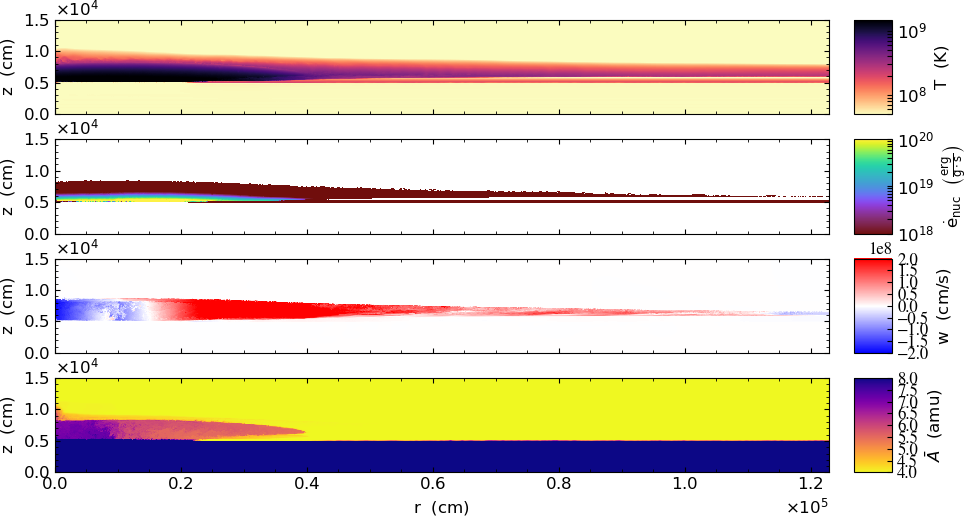
\includegraphics[width=0.95\linewidth]{xrb}
\caption{\label{fig:xrb} Helium flame spreading across the surface of
  a neutron star.  Shown are temperature (top), the mean molecular
  weight of the ash (second), the nuclear energy generation rate
  (third), and the velocity out of the simulation plane (bottom).  The
  out of plane velocity contours indicate where the Coriolis force has
  created a hurricane-like wind structure which confines the flame,
  leading to an inclined front. It is at such an interface that the
  temperature and burning rate are highest.  }
\end{figure}

\section{Large Scale Simulations and Algorithmic Developments}

The 2D calculations shown in the previous section require about 10k
node-hours of computational time to get to about 10~ms (those
particular simulations were run at NERSC).  Most of this time is spent
in the reactions\MarginPar{verify fraction}.  We really need to do 3D.
There the shear from the hurricane structure acting along the flame
front may cause instabilities that can affect the flame propagation.
This is something we can test with our current simulation methodology.
A 3D version of this calculation is estimated to require 5M node-hours
on CPUs---this is about the size of an annual \MarginPar{double check
  \#s} allocation.  Additionally, this is still with the boosted
flame, but we expect that once the flame is developed, the boosting
will not be as critical, due to hydrodynamic effects.  We plan to test
this soon.  We can bootstrap the 3D calculation by mapping the 2D
axisymmetric calculation, once the flame is firmly established, into
3D, rotating about the symmetry axis.  This will cut down the
computational time by about one-half.  In any case, this is less than
1\% of the neutron star surface, so a fully resolved calculation of
burning over the entire neutron star is out of reach, and will be for
some time.

Algorithmic improvements are needed to push the scale of simulations
to the point where we can model XRBs at the full star scale with
resolved nuclear physics.  Here we discuss a few possibilities.

Machine architectures are evolving, with heterogeneous architectures
becoming more common.  Our recent development in \castro\ has focused
on moving the hydrodynamics to GPUs~\cite{astronum:2017}.  The XRB
problem is an ideal case for this, since hydrodynamics with constant
gravity (for plane-parallel domains) ports in a straightforward manner
to GPUs.  The current GPU version of the \castro\ hydrodynamics solver
is about $10\times$ faster using GPUs on a node than the entire node
of CPU cores.  We see similar speed ups with reaction networks, with
these GPU ports under active development.  This means a GPU
calculation could lower the above costs by a factor of 10.  GPU
offloading of the reaction networks will also allow us to explore
larger networks and more detailed nuclear physics.

Another way we can meet the resolution requirements is to use a more
accurate hydrodynamic method.  We are developing fully
fourth-order (in space and time) coupling of hydrodynamics and
reactions using the method of spectral deferred corrections (SDC) in
\castro, instead of the more commonly employed Strang splitting.  This
provides us with two benefits.  First, the improved coupling actually
reduces the stiffness of the reactions, requiring fewer righthand side
calls and therefore reducing the expense of the
reactions. \MarginPar{need some refs here} Second, by moving to fourth
order, we may also be able to reduce our resolution requirements
needed for converged flames, and since computational work scales like
$(\Delta x)^4$ in 3D, this can save a lot of computer time.

As an example of the improvements in coupling between hydro
and \MarginPar{Don can add some comments about startup costs?}
reactions, Figure~\ref{fig:sdc} shows the mass fraction of helium
behind a detonation over the course of 3 timesteps.  The points
represent individual calls to the righthand side function of our
reaction network (a 13-isotope $\alpha$-chain), and the density of
points indicates how hard the integrator is working.  We use the same
tolerances for both the Strang-split method and the SDC method.  For
the SDC method, we are using a second-order accurate method based on
\cite{SDC-old}.  We predict a time-centered advection term,
$\Adv{\Uc}^{n+1/2}_i$ using standard unsplit Godunov methods, but
explicitly include a reactive source term in the tracing of the
interface states, ${\bf R}(\Uc_i)$.  We can then solve the reactive
system, using this advective term as a piecewise-constant-in-time
source
\begin{equation}
\label{eq:syst}
\frac{d{\Uc_i}}{dt} = -\Adv{\Uc}^{n+1/2}_i + {\bf R}(\Uc_i)
\end{equation}
This system can be integrated with standard ODE methods.  To achieve
second-order accuracy, we need to iterate, using the updated $\Uc$ to
create a reactive source included in the predictor for the advective
update, and then reintegrate the system.  The result of this iteration
is that the advection sees the effects of reactions over the timestep
and the reactions see the effects of advection.  For the zone tracked
in Figure~\ref{fig:sdc}, each SDC iteration called the righthand side
function of the network 5 times less than the Strang case.
We are continuing to develop this new integration strategy, with full
fourth-order in space and time reacting hydrodynamics methods to
follow shortly.  The XRB simulations are our target application.

\begin{figure}
\centering
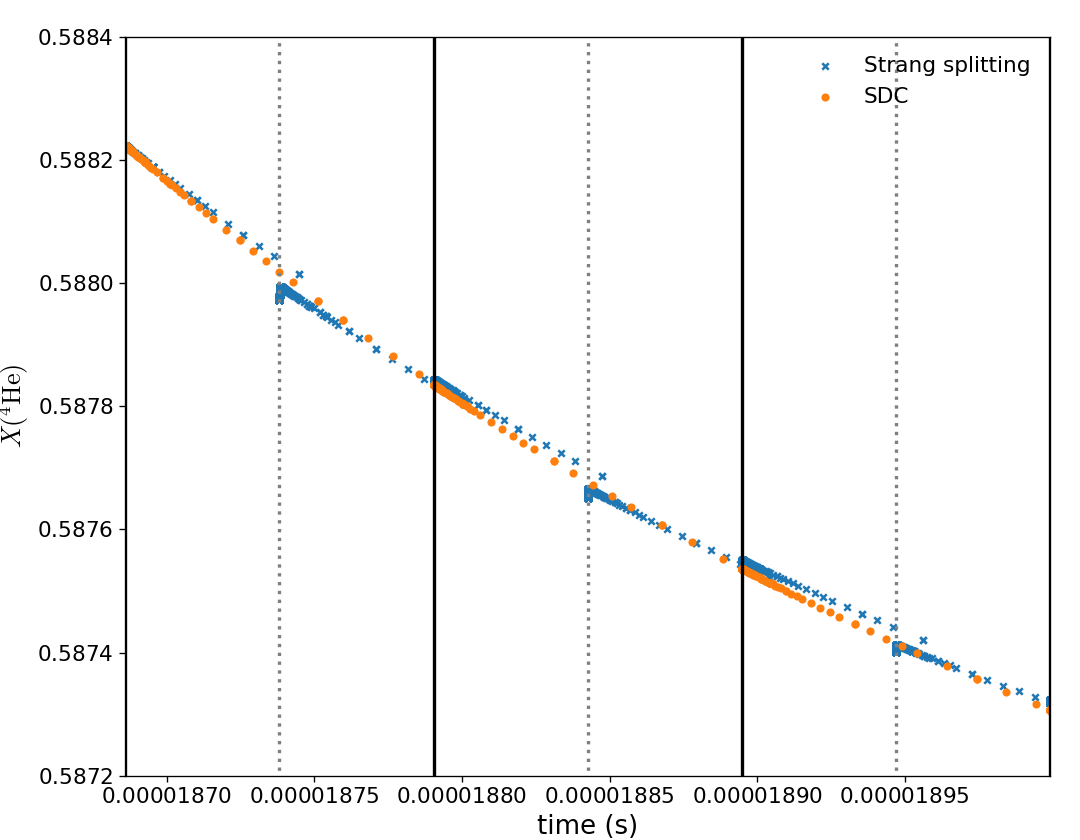
\includegraphics[width=0.75\linewidth]{sdc_plot}
\caption{\label{fig:sdc} Helium mass fraction as a function of time
  over three timesteps.  The points represent individual calls to the
  righthand side function of our reaction network (see
  Eq. \ref{eq:syst}) and the density of points indicates how hard the
  integrator is working.}
\end{figure}

Other ways to make the simulation less expensive can include a subgrid
model. Flame models are commonly used for Type Ia supernovae.  There
however, the flame is thin compared to the scale height, so a simple
model can represent the unresolved flame on the grid.  For the XRB,
the flame thickness is a non-trivial fraction of the pressure scale
height and further, the laminar flame properties will change strongly
over the height of the burning layer (see~\cite{Timmes00}).  This
makes traditional flame models a poor fit.  Methods that use even
something as simple as subzone burning (e.g.~\cite{Wang2012190}) may
help capture the energetics with lower resolution.  This can be
implemented using the AMR machinery.  This may help a little, but will
still be insufficient for full star models.

If we continue to resolve the flame structure, then we need to be
smarter (and more aggressive) about our grid refinement strategy.
Currently, we put the entire fuel layer on the finest grid, but for
the material ahead of the flame, we could keep it at lower resolution
until the flame reaches it.  The main obstacle is that we need to keep
the fuel ahead of the flame in hydrostatic equilibrium, and keeping it
refined accomplishes this well.  Using well-balanced
schemes~\cite{kappeli:2016} can help us retain hydrostatic equilibrium
(HSE) in the lower refined regions, reducing the number of zones
needed to maintain fidelity, but we would still need a way to regrid
the layer ahead of the flame to higher resolution to accurately
capture the burning dynamics.  To accomplish this, we envision
building a refinement strategy that does interpolation of the data onto
the newly refined grids enforcing hydrostatic equilibrium.  This can
allow us to keep only a narrow fully refined region that ``slides''
along the surface of the neutron star keeping pace with the advancing
flame.  Such a scheme would greatly reduce the computational costs.
This is a longer term development.


All of the above developments still involve fully compressible
hydrodynamics, but multiscale methods~\cite{weinan2011principles} where we couple different hydrodynamics
solvers together in a single simulation may ultimately be needed to model the full star while resolving the burning front.
%\MarginPar{Alice and Ian contribute here}
Such techniques rely on it being possible to decompose the dynamics of the system
into two scales, e.g.~a short and a long lengthscale, and that the processes at each
scale are at most weakly coupled with each other. In the context of XRBs, one possibility for
multiscale modelling would be to model the large scale dynamics using a shallow water model
(like that of~\cite{SPIT_ETAL02}) to capture the effects of the Coriolis force, and use
a low Mach number or
a fully compressible model in the vicinity of the burning front to capture
the turbulent burning processes. Given that the computational costs of the 2D shallow water model
would be negligible compared to those of the low Mach/compressible model, the overall cost of
this multiscale model would be determined by the size of the low Mach/compressible region only. This
approach would therefore allow us to capture dynamics across the full star
without sacrificing resolution around the flame.
An example of coupling compressible and low Mach number models implemented using the \amrex~framework, but in a terrestrial context,
is~\cite{Motheau2018}. An initial implemenation, \cite{Harpole2018}, in an
astrophysical context, coupling shallow water to compressible models in both
Newtonian and relativistic gravity, indicates that considerable computational
efficiencies are possible, but that close attention to the coupling between the
models is needed.

%% Finally, we can try hybrid model approaches where the fully
%% compressible simulation can act as a subgrid model.
%% Multiscale methods can combine different hydro models together to allow
%% for a full star simulation with resolved burning.  Examples include...


\section{Summary}

\ack The work at Stony Brook was supported by DOE/Office of Nuclear
Physics grant DE-FG02-87ER40317 and contract 7418390 with Lawrence
Berkeley National Laboratory as part of the Exascale Compute Project
ExaStar collaboration.  The work at LBNL was supported by the DOE
Office of Advanced Scientific Computing Research under Contract No,
DE-AC02-05CH11231. YC is supported by the European Union Horizon 2020
research and innovation programme under the Marie Sklodowska-Curie
Global Fellowship grant agreement No 703916.  An award of computer
time was provided by the Innovative and Novel Computational Impact on
Theory and Experiment (INCITE) program. This research used resources
of the Oak Ridge Leadership Computing Facility at the Oak Ridge
National Laboratory, which is supported by the Office of Science of
the U.S. Department of Energy under Contract No.\ DE-AC05-00OR22725.
This research used resources of the National Energy Research
Scientific Computing Center, which is supported by the Office of
Science of the U.S. Department of Energy under Contract
No.\ DE-AC02-05CH11231.  Visualizations were done using yt~\cite{yt}.
This research has made use of NASA's Astrophysics Data System
Bibliographic Services.


\section*{References}

\bibliographystyle{iopart-num}
\bibliography{ws}


\end{document}
